\documentclass[8pt, landscape, a4paper]{extarticle}

% --- 核心宏包 ---
\usepackage[UTF8]{ctex}
\usepackage[margin=0.8cm, top=1cm, bottom=1.3cm]{geometry}
\usepackage{multicol}
\usepackage{xcolor}
\usepackage{tcolorbox}
\usepackage{enumitem}
\usepackage{amsmath}
\usepackage{amssymb}
\usepackage{fontspec}
\usepackage{tikz}
\usetikzlibrary{arrows.meta, shapes}

% --- 去掉页码 ---
\pagestyle{empty}

% --- 颜色定义 (Maroon 主题) ---
\definecolor{headerblue}{RGB}{128, 0, 0}       % Maroon
\definecolor{navcolor}{RGB}{211, 84, 0}        % 导航橙
\definecolor{intuitioncolor}{RGB}{41, 128, 185}% 直觉蓝
\definecolor{accentcolor}{RGB}{230, 126, 34}   % 强调橙
\definecolor{section2}{RGB}{22, 160, 133}      % 绿色
\definecolor{dividergray}{RGB}{220, 220, 220}

% --- 全局设置 ---
\setlength{\parindent}{0pt}
\setlength{\columnsep}{0.4cm} 
\linespread{1.1} 

% --- 列表样式 ---
\setlist[itemize]{leftmargin=1.2em, nosep, itemsep=2pt, topsep=2pt, label=$\textcolor{headerblue}{\vcenter{\hbox{\tiny$\bullet$}}}$ }
\setlist[description]{leftmargin=0.2em, style=sameline, nosep, itemsep=2pt, font=\bfseries}

% --- Box 样式 ---
\newtcolorbox{mybox}[2][]{%
  colback=white,
  colframe=#2,
  coltitle=white,
  boxrule=1pt,             
  arc=2mm,                 
  left=4pt, right=4pt, top=3pt, bottom=3pt, 
  toptitle=3pt, bottomtitle=3pt, 
  fonttitle=\bfseries\sffamily\large,
  title={#1},
  after skip=5pt          
}

% --- 自定义命令 ---
\newcommand{\subt}[1]{{\vspace{2pt}\textbf{\large \textcolor{black}{#1}}}}

\newcommand{\boxdesc}[1]{%
    \textit{\small \textcolor{gray}{#1}}%
    \par\vspace{2pt}%
    {\color{dividergray}\hrule height 0.5pt}%
    \vspace{2pt}%
}

\newcommand{\sepline}{%
    \par \vspace{3pt}%
    {\color{dividergray}\hrule height 0.5pt}%
    \par \vspace{3pt}%
}

% 公式间距
\setlength{\abovedisplayskip}{3pt}
\setlength{\belowdisplayskip}{3pt}

\begin{document}

% --- 页眉 ---
\begin{center}
    {\Huge \textbf{\sffamily \textcolor{headerblue}{代数几何 Algebraic Geometry Cheat Sheet}}} \\
    \vspace{0.2cm}
    {\large \texttt{Geometry of Equations: Varieties, Schemes, and Cohomology}}
\end{center}

% --- 开始四栏布局 ---
\begin{multicols*}{4}

% === 第一栏 ===

\begin{mybox}[️ 场景导航 (Use Cases)]{navcolor}
    \boxdesc{遇到什么问题 $\to$ 用什么工具}
    \begin{itemize}[itemsep=2pt]
        \item \textbf{机器人运动学} $\to$ 理想/Gröbner 基
        \item \textbf{密码学 (ECC)} $\to$ 椭圆曲线
        \item \textbf{纠错码} $\to$ Goppa 码 / 代数曲线
        \item \textbf{计算机视觉} $\to$ 射影几何 / 基础矩阵
        \item \textbf{系统生物学} $\to$ 化学反应网络理论
        \item \textbf{字符串理论} $\to$ Calabi-Yau 流形
    \end{itemize}
\end{mybox}

\begin{mybox}[1. 仿射簇 (Affine Varieties)]{headerblue}
    \boxdesc{多项式的零点集}
    
    \subt{定义 $V(S)$}
    给定多项式集合 $S \subset k[x_1, \dots, x_n]$,
    $$ V(S) = \{x \in k^n \mid f(x) = 0, \forall f \in S\} $$
    \sepline
    
    \subt{理想 (Ideal) $I(V)$}
    在 $V$ 上全为 0 的多项式集合。
    \sepline
    
    \subt{希尔伯特零点定理 (Nullstellensatz)}
    代数与几何的完美对应 (在代数闭域上):
    $$ I(V(J)) = \sqrt{J} $$
    \textit{几何对象 (簇) 与代数对象 (理想) 一一对应。}
\end{mybox}

\begin{mybox}[2. 射影几何 (Projective)]{headerblue}
    \boxdesc{引入无穷远点}
    
    \subt{射影空间 $\mathbb{P}^n$}
    $k^{n+1} \setminus \{0\}$ 中过原点的直线集合。
    坐标 $(x_0 : x_1 : \dots : x_n)$,差一个缩放因子。
    \sepline
    
    \subt{齐次多项式}
    只有齐次多项式在射影空间上有定义 (零点位置不变)。
    \sepline
    
    \subt{贝祖定理 (Bézout)}
    两条 $m$ 次和 $n$ 次的平面曲线,在 $\mathbb{P}^2$ 中恰好有 $mn$ 个交点 (计入重数)。
    \textit{完美!没有“平行线不相交”这种例外。}
\end{mybox}

\columnbreak

% === 第二栏 ===

\begin{mybox}[3. 概型 (Schemes)]{headerblue}
    \boxdesc{格罗滕迪克的革命}
    
    \subt{为什么需要概型?}
    簇无法处理重根 (如 $x^2=0$) 和数论问题 (整数环 $\mathbb{Z}$)。
    \sepline
    
    \subt{仿射概型 Spec(R)}
    环 $R$ 的所有\textbf{素理想}构成的空间。
    \textit{包含了几何点 (极大理想) 和“肥点” (非极大素理想)。}
    \sepline
    
    \subt{层 (Sheaf) $\mathcal{O}_X$}
    在每个开集上定义“函数”。
    概型 = 拓扑空间 + 结构层 (局部像 Spec(R))。
\end{mybox}

\begin{mybox}[4.  Gröbner 基 (Gröbner Basis)]{headerblue}
    \boxdesc{多项式的“高斯消元”}
    
    \subt{问题}
    如何判断 $f$ 是否属于理想 $I = \langle f_1, \dots, f_m \rangle$?
    如何解多项式方程组?
    \sepline
    
    \subt{Buchberger 算法}
    计算理想的一组“好”的生成元 $G$。
    \begin{itemize}
        \item 任意多项式除以 $G$ 的余式唯一。
        \item 可以用来消元、解方程。
    \end{itemize}
    \textit{计算代数几何的核心算法。}
\end{mybox}

\columnbreak

% === 第三栏 ===

\begin{mybox}[5. 椭圆曲线 (Elliptic Curves)]{headerblue}
    \boxdesc{代数几何的明珠}
    
    \subt{方程}
    $$ y^2 = x^3 + ax + b $$
    \sepline
    
    \subt{群结构}
    曲线上的点构成一个阿贝尔群。
    \textbf{加法法则}: 三点共线 $P+Q+R=0$ (几何作图)。
    \sepline
    
    \subt{应用}
    \begin{itemize}
        \item \textbf{ECC}: 离散对数问题难解。
        \item \textbf{费马大定理}: 证明的核心。
    \end{itemize}
\end{mybox}

\begin{mybox}[6. 奇点理论 (Singularities)]{headerblue}
    \boxdesc{光滑性的破坏}
    
    \subt{光滑点}
    雅可比矩阵满秩的点。
    \sepline
    
    \subt{奇点消解 (Resolution)}
    广中平祐定理:特征 0 域上的任意代数簇都可以通过“吹爆” (Blow-up) 变成光滑的。
\end{mybox}

\begin{mybox}[7. Python / SageMath 实战]{headerblue}
    \boxdesc{代码工具箱}
    \begin{itemize}
        \item \textbf{SageMath}: 最强开源数学软件。
        \item \texttt{R.<x,y,z> = PolynomialRing(QQ)}
        \item \texttt{I = R.ideal([x^2+y^2-1, x-y])}
        \item \texttt{I.groebner\_basis()}
        \item \texttt{E = EllipticCurve([a, b])}
    \end{itemize}
\end{mybox}

\columnbreak

% === 第四栏 ===

\begin{mybox}[8. 高阶前沿 (Advanced)]{headerblue}
    \boxdesc{深空探索}
    
    \subt{模空间 (Moduli Space)}
    参数化一族几何对象的空间。
    \textit{例: 所有亏格为 $g$ 的黎曼面的集合 $\mathcal{M}_g$。}
    \sepline
    
    \subt{平展上同调 (Etale Cohomology)}
    为了证明韦伊猜想 (Weil Conjectures) 而发明的。
    在代数几何中定义了类似拓扑学的“孔”。
    \sepline
    
    \subt{Motive (动机)}
    格罗滕迪克的终极梦想:统一所有上同调理论。
\end{mybox}

\vspace*{\fill}

\begin{mybox}[ 核心直觉 (Intuition)]{intuitioncolor}
    \boxdesc{“代数是几何的影子。”}
    
    % TikZ 矢量图: 椭圆曲线加法
    \begin{center}
    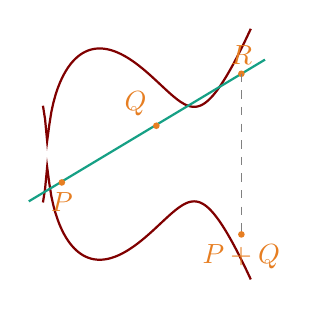
\begin{tikzpicture}[scale=0.6]
        % 椭圆曲线 (示意)
        \draw[thick, headerblue, domain=-2.2:2.2, samples=100] plot (\x, {sqrt(abs(\x^3 - 3*\x + 3))});
        \draw[thick, headerblue, domain=-2.2:2.2, samples=100] plot (\x, {-sqrt(abs(\x^3 - 3*\x + 3))});
        
        % 直线
        \draw[section2, thick] (-2.5, -1) -- (2.5, 2);
        
        % 交点 P, Q, R
        \fill[accentcolor] (-1.8, -0.6) circle (2pt) node[below] {$P$};
        \fill[accentcolor] (0.2, 0.6) circle (2pt) node[above left] {$Q$};
        \fill[accentcolor] (2.0, 1.7) circle (2pt) node[above] {$R$};
        
        % R' (P+Q)
        \draw[dashed, gray] (2.0, 1.7) -- (2.0, -1.7);
        \fill[accentcolor] (2.0, -1.7) circle (2pt) node[below] {$P+Q$};
        
    \end{tikzpicture}
    \end{center}

    \hspace{1em}代数几何在\textbf{方程} (代数) 和\textbf{形状} (几何) 之间建立了字典。
    \vspace{4pt}
    
    \subt{三大核心视角}
    \begin{itemize}[itemsep=4pt]
        \item \textbf{刚性}: 
        代数函数 (多项式) 非常坚硬。如果你知道它在局部的一小段,你就知道了它在全宇宙的样子 (解析延拓)。这与拓扑学的柔软形成鲜明对比。
        
        \item \textbf{内蕴代数}: 
        坐标环 $k[V]$ 包含了簇 $V$ 的所有几何信息。研究几何变成了研究环论。
        
        \item \textbf{无穷远点}: 
        射影几何告诉我们,平行线在无穷远处相交。这修复了欧几里得几何中的许多“例外”,让定理变得完美 (如 Bézout 定理)。
    \end{itemize}
    
    \vspace{6pt}
    \centering\textit{\footnotesize 每一个素理想都是一个点,每一个环都是一个世界。}
\end{mybox}

\end{multicols*}

\end{document}
